\chapter{Literature Review}
\label{chap:Two}

Following the initial work done by Axelrod, there are many other papers that
have tried to tackle the PD and make their conclusions on cooperation in both a
theoretical and real life setting. In this chapter a review of some of this work
done in the IPD competitions, in spatial and evolutionary game theory will be
carried out.

\section{Tournaments}

In order to identify the condition under which cooperation could emerge
in the game of the Prisoner's Dilemma better, Robert Axelrod held a tournament
in 1980. He invited a number of well-known game theorists to submit strategies
for a computer tournament.  Each strategy has to specify whether to cooperate or
defect based on the history of previous moves made by both players.
Strategies played again
each other as well as a further Random strategy, that would randomly choose
between C and D and with its own twin (same strategy). The tournament was a
round robin with the payoff matrix~\ref{fig:pd_payoff}. All entries knew the
exact length (200 moves) of each game. To improve the reliability of the scores
the entire round robin tournament was repeated five times. Fourteen strategies were
submitted and by the end Tit for Tat was announced the winner. Surprisingly in
the second tournament held where 64 strategies competed and all submitters had
full knowledge of what have happened in the first tournament, Tit for Tat
managed to get first place again\cite{Axelrod1980a}.

As explained in \cite{Axelrod1980b}, Tit for Tat, a simple strategy was
able to beat sophisticated and more complex strategies thanks to three
specific characteristics of the strategy:

\begin{itemize}
  \item Niceness:  A strategy is categorized as nice if it was not the
                    first to defect, or at least, it will not do this until
                    the last few moves.
  \item Forgiveness: The propensity to cooperate in the moves after the
                     opponent defected.
  \item Clarity: After opponents identified that they were playing Tit for Tat
                 choose to cooperate for the rest of the game.
\end{itemize}

The first tournaments were an innovation in combining computer modeling and Game
Theory and in providing insights in the behavior emerging from simple dynamics.
Moreover, Axelrod was the first to speak about niceness, forgiveness and gave an
illustration that cooperation can be a victorious and advantageous strategy.

Another concept that had been developed was the Evolutionary Game Theory (EGT).
EGT is an application of game theory to biological contexts, arising from the
realization that frequency dependent fitness introduces a strategic aspect to
evolution. In 1973, Maynard and Price introduced the concept of Evolutionary
Stable Strategy (ESS), which is an extension of a Nash Equilibrium. If a
population of the same strategies cannot be invaded by any alternative strategy
that is initially rare then that strategy is an ESS. In his third tournament
Axelrod \cite{Axelrod1981} using the same set of strategies (63),
the tournaments introduced a dynamical rule that mimics Darwinian selection.
In this evolutionary computer tournament after a round robin game the score for
each player was evaluated, and the strategies with high score would be adapted
while the lowest ones ones would diminish. In most of these simulations, the
success of Tit-for-Tat was confirmed because the population would end up with
some mutually cooperating strategies prevailed by Tit-for-Tat.

There have been other tournaments, based off of Axelrod’s, exploring different
environments and submitting new strategies. Boyd \& Lorderbaum \cite{Lorberbaum1994}
state that no pure
strategy is evolutionary stable because each can be invaded by the joint effect
of two invading strategies when long term interaction occurs in th repeated game
and future moves are discounted. In 1991 Bendor, Kramer and Stout \cite{The2016}
introduced noise to the IPD. Where noisy randomly flip the choice made by a
strategy. The results of their tournament was that the strategies that were more
generous, cooperated more than their opponents did, were more effective than Tit
for Tat. Moreover, Kerts 2011 conducted a tournament where the payoff matrix was
altered though satisfying the conditions \ref{firstassum}, \ref{secondassum}.

Furthermore, two more notable tournaments took place in 2005 and 2012.
In the 2005 IPD competition a team from the University of Southampton participated
using a group of strategies which won the top three propositions. These strategies
were designed in such why that thought a predetermined sequence of five to ten
moves would recognize each other. Once the two Southampton players recognized
each other they would take up the roles of a ruler and a slave. The ruler
would always cooperate where the slave would defect in order to maximize the
payoff of the ruler. If the opponent was recognized to not being one of the team
then the Southampton player would always choose to defect to minimize the score
of the opponent \cite{Li2011}. Lastly, the Stewart- Plotkin \cite{Stewart2012}
tournament which
consisted of nineteen strategies, including a new set of strategies; the Zero-
determinant(ZD) strategies. The ZD are strategies for the stochastic iterated
prisoner's dilemma, discovered by Press and Dyson in 2012 \cite{Press2012a}.
The ZD apply a linear relationship between their own payoff and that of the opponent.
Some review tournaments are listed on the Table~\ref{tab:tournaments}:

\begin{table}[!hbtp]
    \begin{center}
        \begin{tabular}{ccccc}
            \toprule
            Year     & Reference                  & Number of Strategies & Type     \\
            \midrule
            1979     & \cite{Axelrod1980a}        & 13                   & Standard  \\
            1979     & \cite{Axelrod1980b}        & 64                   & Standard  \\
            1984     & \cite{Axelrod1981}         & 64                   & Evolutionary\\
            1991     & \cite{The2016}          & 13                   & Noisy     \\
            2005     & \cite{Chong2004} & 223                  & Varied    \\
            2012     & \cite{Stewart2012}         & 13                   & Standard   \\
            \bottomrule
        \end{tabular}
    \end{center}
    \caption{An overview of a selection of published tournaments.}\label{tab:tournaments}
\end{table}

In this section the work done for tournaments in the IPD has been cited and analyzed.
Starting with the the work of Axelrod, the reasons the tournaments where organized
and what where the fundings. Moreover, some research that has been generated the following
years are stated. Below, a specialized case of these research will be studied. That
case is that of the spatial structure tournaments.

\section{Spatial Structure Tournaments}

Further research was spawn in 1992 as to how the Prisoner's Dilemma could shade
some insight into physics and biology. Where Nowak and May believed exist potential
dynamics of spatially extended systems. Their tournament was a simple and purely
deterministic spatial version of the PD in a two dimensional lattice. With
players having no memory of the previous rounds and no strategical elaboration.
Thus, the players could either always cooperate or defect. In each round each
player interact with the immediate neighbor. \footnote{In Nowak's and May's
experiment, the result's hold for all three cases that  the player interacts with
4, 6 and 8 neighbors.} They used an evolution rule that after each round
round the nodes with the lowest score in their neighborhood would copy the
strategy of the player with the highest score. This was done to study which
behavior, defection or cooperation , would last. The conclusion was that co-operational
behavior is possible in the PD by using a spatial topology. Nowak produced more
work on the topic on papers of his such as \cite{Nowak1993} (Nowak 1994).
In his subsequent papers Nowak et al. (1994a,b)  different spatial structures
where studied. Including triangular and cubic lattices and a random grid.
It turned out that cooperation can be maintained in spatial models even
for some randomness.

On the other hand,  in \cite{Lindgren1994} players were allowed to have
memory and therefore added complex strategies to the tournament such as Tit for
Tat and  Anti Tit for Tat. This was followed  by the work of
\cite{Brauchli1999} which introduced even more complex strategies. Brauchli et
all compares the spatial model with a randomly mixed model.
A more complex strategy that they have tested was PAVLOV. A win-stay,
lose-switch strategy.  According to their
fundings, there is more cooperative behavior in a spatial structure tournament
and evolution is more less chaotic than in unstructured populations. Also as
stated, generous variants of PAVLOV are found to be very successful
strategies in playing the Iterated Prisoner's Dilemma.

Spatial topology has been defined by most scholars as a square lattice where
the nodes - players only interact with their neighborhoods. Including connections
between four or eight nearest neighbor sites, Neuman's or Moore's, according to
Figure~\ref{fig:neighborhood}. A square lattice is a graph and one could argue
that a round robin tournament itself is the complete graph on all players
\cite{Bela}. But in the above papers
no authors defined the topology as a graph, apart from \cite{Meng2015}.

In \cite{Meng2015}, an interesting approach was used. They presented a new
spatial prisoner's dilemma game model in which the neighborhood size was
increased onto two interdependent lattices. They implement the utility by
integrating the payoff correlations between two lattices. A player would mimic a
random player in his next move, base on a function that consider the utility of
the player. It was characterized as a most realistic scenario.

Real life interactions are more likely to be like any given graph depending on
the industry than a complete graph. Fatha et all \cite{Szabo2007}, have
considered a numerous of graphs, such as :

\begin{itemize}
  \item Lattice, the interaction network is defined by the sites of a lattice.
   the distance between a pair does not exceed a given value.
   The most frequently used structure is the square lattice with von Neumann
   neighborhood and Moore neighborhood.
  \item Small word, a graph that is created from a square lattice by randomly
   rewiring a fraction of connections in a way that conserve the degree for
   each site.
  \item Scale-free graphs, a network that has a power-law degree distribution, regardless of
   any other structure.
  \item Evolving networks, networks that change as a function of time (this will
      not be considered in this dissertation).
\end{itemize}

The major theme of their review was how the graph structure of interactions could
modify long term behavioral patterns emerging in evolutionary games.
These graphs compose only a small fraction of graphs that exist. In this
dissertation we will consider a list of graphs.
 %add list when i actually know

\section{Axelrod Python Library}

The Axelrod library \cite{axelrodproject} is an open source Python package that allows for
reproducible game theoretic research into the Iterated Prisoner's Dilemma
\url{https://github.com/Axelrod-Python}.
For many of the tournaments aforementioned the original source code is almost never
available and in no cases is the available code well-documented, easily modified
or released with significant test suites. Due to that reproducing the results
has not been an easy task.

However, Axelrod library manages to provide such a resource, with facilities for
the design of new strategies and interactions between them, as well as
conducting tournaments and ecological simulations for populations of strategies.

Strategies are implemented as classes which have a single method, \texttt{strategy()}.
It only takes one argument, which is the opponent's previous moves and returns
an action. These actions can be either to cooperate C or to defect D. At thins
moment the Axelrod library consists of 131 strategies.Can be found in the Appendix.
As an example we can see in Figure  the source code for the
famous strategy Tit for Tat.

\begin{listing}[H]
\usemintedstyle{tango}
\begin{minted}
[
frame=lines,
framesep=2mm,
baselinestretch=1.2,
bgcolor=LightBlue,
fontsize=\footnotesize,
linenos
]
{python}

class TitForTat(Player):
    """
    A player starts by cooperating and then mimics
    the previous action of the opponent.

    Note that the code for this strategy is written
    in a fairly verbose way. This is done so that it
    can serve as an example strategy for those who
    might be new to Python.
    """

    # These are various properties for the strategy
    name = 'Tit For Tat'
    classifier = {
        'memory_depth': 1,  # Four-Vector = (1.,0.,1.,0.)
        'stochastic': False,
        'makes_use_of': set(),
        'inspects_source': False,
        'manipulates_source': False,
        'manipulates_state': False
    }

    def strategy(self, opponent):
        """This is the actual strategy"""
        # First move
        if len(self.history) == 0:
            return C
        # React to the opponent's last move
        if opponent.history[-1] == D:
            return D
        return C
\end{minted}
\caption{Tit for Tat source code.}
\end{listing}

Additionally, tournament is a class responsible for coordinating the play of
generated matches. It achieves that by calling a match generator class which
returns all the single match parameters, such as turns, the game and the noise.
Axelrod has the capability to write out the results into a csv file and also out
put plots with the ranks of the strategies.

Furthermore, a basic tournament of 200 turns, 100 repetitions and the 131
strategies that exist in the library is being produced continuously. The current
winner is called PSO gambler and it is a look up strategy. It uses a lookup
table with probability numbers generated using a Particle Swarm Optimisation
(PSO) algorithm, the sourse code can be found here :
 \url{http://axelrod.readthedocs.io/en/latest/_modules/axelrod/strategies/gambler.html?highlight=Gambler})
 and a description of how this strategy was trained is given here:
 \url{https://gist.github.com/GDKO/60c3d0fd423598f3c4e4}.
It uses a 64-key lookup table (keys are 3-tuples consisting of the opponent's
starting actions, the opponent's recent actions, and our recent action) to
decide whether to cooperate (C) or defect (D). The actions for each key were
generated using an evolutionary algorithm.

To reproduce a basic tournament with the 131 strategies using Axelrod :

\begin{listing}[ht]
\begin{minted}
[
frame=lines,
framesep=2mm,
baselinestretch=1.2,
bgcolor=LightGray,
fontsize=\footnotesize,
linenos
]
{python}

>>> import axelrod
>>> strategies = [s() for s in axelrod.ordinary_strategies]
>>> tournament = axelrod.Tournament(strategies)
>>> results = tournament.play()
>>> plot = axelrod.Plot(results)
>>> p = plot.payoff()
>>> p.show()
\end{minted}
\caption{A simple set of commands to create a basic tournament. The
    output is shown in Figure~\ref{fig:axelrodplots}.}
\end{listing}

 Here are illustrated the results of the last tournament :
 \newpage

\begin{figure}[h]
\centering
    \begin{subfigure}[t]{0.7\textwidth}
    \centering
        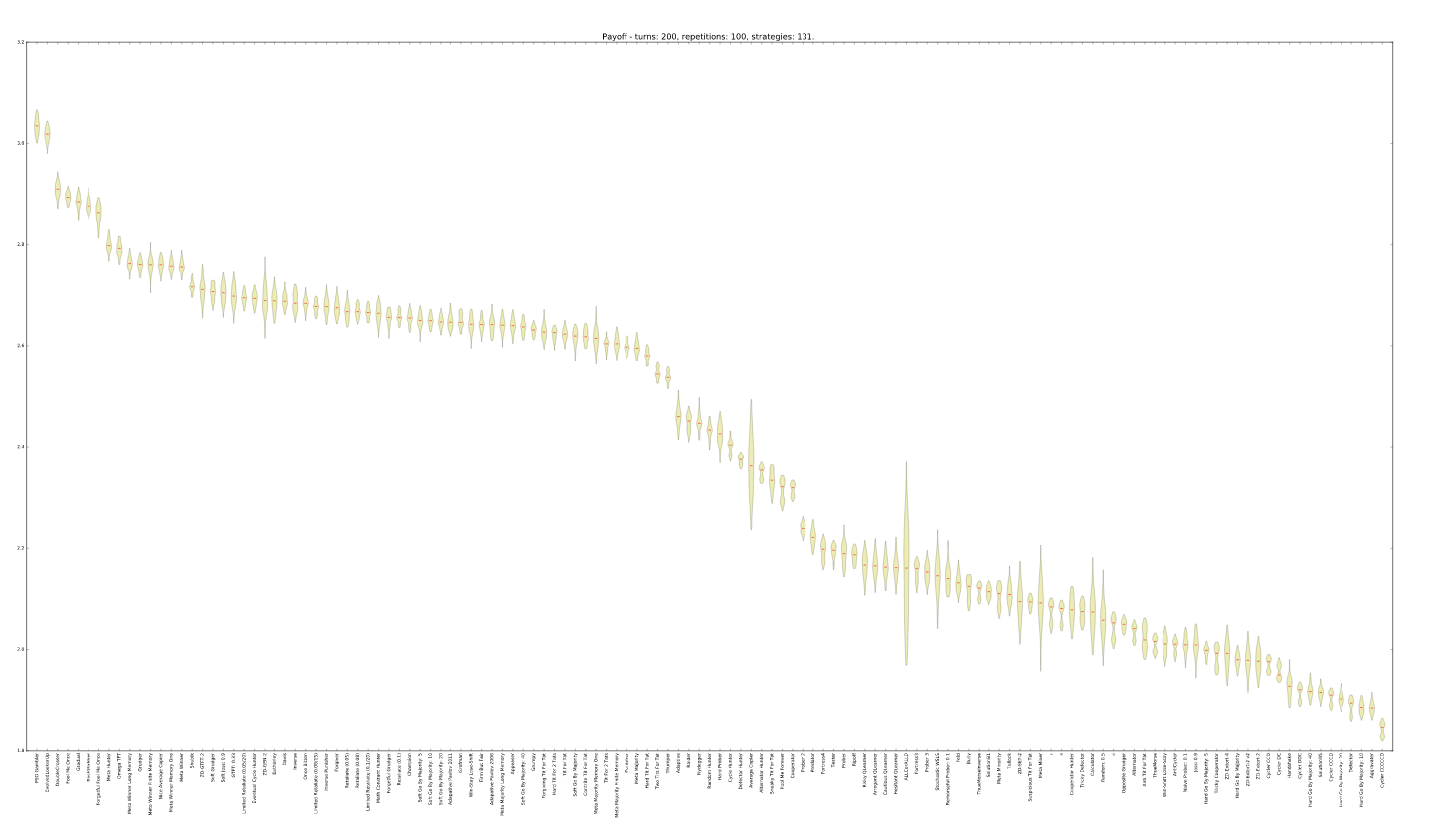
\includegraphics[width=\linewidth]{axl.png}
    \caption{Ranked violin plot}
    \end{subfigure}
\hfill
    \begin{subfigure}[t]{0.70\textwidth}\centering
    \centering
        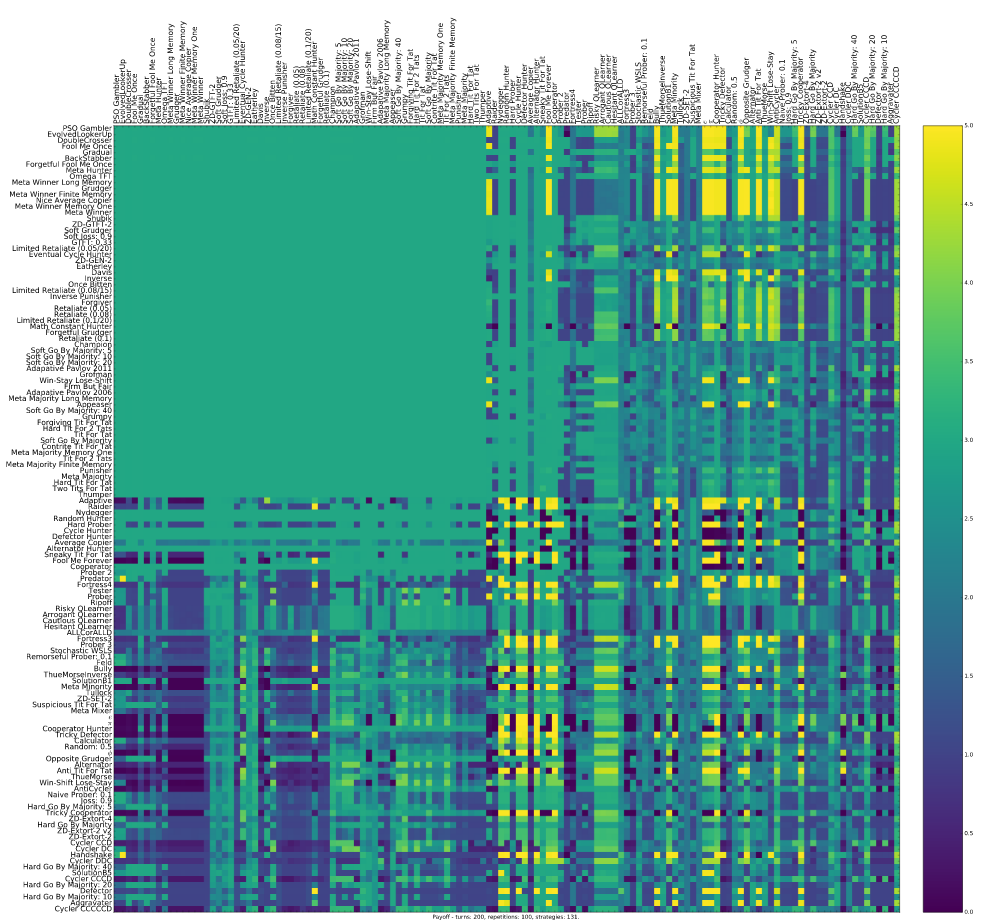
\includegraphics[width=\linewidth]{axl1.png}
    \caption{Payoffs}
    \end{subfigure}
~
\caption{Result Plots. (a) Ranked violin plot, the mean utility of each player.
(b) Payoffs, the pair wise utilities of each player.}
\label{fig:axelrodplots}
\end{figure}

More details for the documentation of the library can be found here :
\url{https://axelrod.readthedocs.io/en/latest/index.html}.
Because is an open source library it makes it easy to contribute to it and
make modifications needed for this dissertation.
